\documentclass[a4paper,12pt,titlepage]{report}

\usepackage[utf8]{inputenc}
\usepackage[T1]{fontenc}
\usepackage[francais]{babel}
\usepackage{mathtools,amssymb,amsthm}
\usepackage[top=20mm, bottom=25mm, left=15mm, right=15mm]{geometry}

\newcommand{\octave}{\textit{Octave }}

\title{Rapport d'Avancement Projet Signal\\Reconnaissance Optique de Caractères}
\author{Tristan DRUSSEL - Florian POUTHIER \\ \\ Génie Électrique - 4ème année\\ INSA Strasbourg}
\date{Année scolaire 2019-2020}

\begin{document}
	\begin{titlepage}
		\maketitle
	\end{titlepage}
	\tableofcontents
	\newpage
	\section*{Introduction}
		Dans le cadre du cours de signal dispensé au semestre 8 de la formation en Génie Électrique, nous devons réaliser un projet utilisant les compétences et connaissances acquises dans le cours mais aussi approfondir dans le domaine qui concerne notre sujet.
		Notre sujet est la \textit{Reconnaissance Optique de Caractères (ROC)}. Avec les méthodes et les outils de traitement du signal, nous allons pouvoir comparer des caractères et ainsi transformer une photo en un fichier texte numérique.
		\subsection{Une image, un signal?}	
		La première des choses est de définir l'image. Une image en informatique est un tableau où l'image est découpée en petits carrés. Chaque case du tableau correspond à un petit carré de l'image et le contenu du tableau est la quantité de rouge, de vert et de bleu de chaque découpage. Plus il y a de découpage plus l'image est précise.
		Afin que l'image devienne un objet mathématique nous pouvons la transformer en une matrice, le tableau défini précédemment peut donc devenir la matrice suivante:
		\begin{equation}
		\begin{bmatrix} 
		\begin{pmatrix} r \\ g\\ b \end{pmatrix} &\begin{pmatrix} r \\ g\\ b \end{pmatrix}&\begin{pmatrix} r \\ g\\ b \end{pmatrix} 
		\\ \begin{pmatrix} r \\ g\\ b \end{pmatrix} & \begin{pmatrix} r \\ g\\ b \end{pmatrix}&\begin{pmatrix} r \\ g\\ b \end{pmatrix}
		\\ \begin{pmatrix} r \\ g\\ b \end{pmatrix} & \begin{pmatrix} r \\ g\\ b \end{pmatrix}&\begin{pmatrix} r \\ g\\ b \end{pmatrix} 
		\end{bmatrix}
		\end{equation}
		Cette matrice de $ M_{m,n}([0,255]^3)$ permet donc de représenter n'importe quelle image et a autant de coefficients que l'image est décomposée en petites cases.
		Cette écriture est pratique, en effet nous avons accès à chaque proportion de couleur de chaque découpage. En revanche travailler avec des matrices de vecteurs n'est pas chose simple. Nous allons donc transformer cette matrice en une matrice d'éléments de $I=[0,255]$. Pour cela nous avons plusieurs solutions, nous pouvons créer une image en nuance de rouge, on ne prend que la première composante du vecteur de chaque case, en nuance de vert, en prenant la seconde, en nuance de bleu en prenant la dernière ou encore en nuance de gris. Cette dernière s'obtient en faisant la moyenne des scalaires $r$,$g$ et $b$ de chaque vecteur. Nous obtenons donc une matrice de $M_{(m,n)}(I)$:
		\begin{equation}
		\begin{bmatrix} 
		\bar{x} & \bar{x} & \bar{x} 
		\\  \bar{x} & \bar{x} & \bar{x} 
		\\  \bar{x} & \bar{x} & \bar{x}
		\end{bmatrix}
		\end{equation}
		Nous obtenons donc une matrice plus simplement exploitable avec les techniques de traitement du signal.
		\subsection{La corrélation}
		La \textbf{corrélation} est une fonction mathématique qui mesure le degré de ressemblance entre un signal original et une version translatée et/ou bruitée de celui ci. On peut définir cette fonction par la relation suivante:
		\begin{equation}
			C(\tau)=\int_{-\infty}^{+\infty}s(t)r(t-\tau)dt \text{ avec s et r signaux quelconque}
		\end{equation}
		Nous pouvons traduire cette expression pour des signaux discrets.
		\begin{equation}
			C(n)=\sum_{-\infty}^{+\infty}s(k)r(k-n)	
		\end{equation}		
		Ces deux définitions sont valables pour des signaux à une dimension comme des signaux temporels. Nos images sont des signaux bidimensionnels avec une variation en $x$ et en $y$.
		\begin{equation}
			C(x,y)=\sum_{x,y} I_1(n,k)I_2(n-x,k-y) \text{ avec}I_1, I_2 \text{ les images}
		\end{equation}
		En calculant les coefficients de corrélation pour toutes les possibilités, nous pouvons déterminer les "endroits" où les deux signaux se ressemblent le plus.
		Les commandes \octave permettant de calculer ces coefficients sont:
		\begin{itemize}
		\item \texttt{corr2}, du paquet \texttt{image}, permettant de calculer les coefficients entre deux images
		\item \texttt{xcorr2}, du paquet \texttt{signal}, permettant de calculer la corrélation 2D entre deux matrices
		\item \texttt{normxcorr2}, du paquet \texttt{image}, permettant de calculer les coefficients de corrélation normalisés entre deux images. 
		\end{itemize}		
		La corrélation est un outil fonctionnant beaucoup mieux sur des fonctions à valeurs moyennes nulles.
	\section{Solutions}
	Nous allons écrire un script \octave qui permet dans un premier temps de charger un motif et une autre image dans le but de chercher ce motif dans l'image. Nous pouvons décomposer notre script en plusieurs étapes: Charger et mettre en forme les images, chercher le motif dans l'image et finalement afficher la localisation.
	\subsection{L'image}
	Avant de vouloir exploiter des images, nous devons tous d'abord les créer. Nous allons donc sur un logiciel de dessin numérique et nous créons deux images, un motif et une image contenant une ou plusieurs fois ce motif.\\
		\begin{tabular}{|c|c|}
			
\includegraphics{../motif.png} & 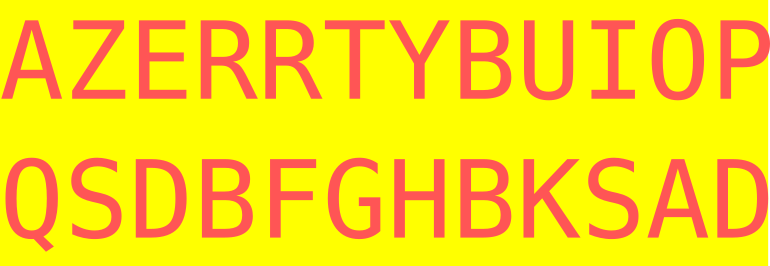
\includegraphics{../mot.png}\\
			Motif créé  & Image globale\\
		\end{tabular}\\
	Nous importons les images dans \octave et nous les convertissons en une matrice de matrice, nous récupérons ensuite l'image en niveau de gris. La dernière étape avant de pourvoir appliquer l'intercorrélation sur les images, il faut transformer les signaux en signaux à valeurs moyennes nulles, nous enlevons donc la valeur moyenne de la matrice à chaque élément.\\
	\begin{tabular}{|c|c|}
			
\includegraphics[scale=0.18]{illus/motifm0.png} & 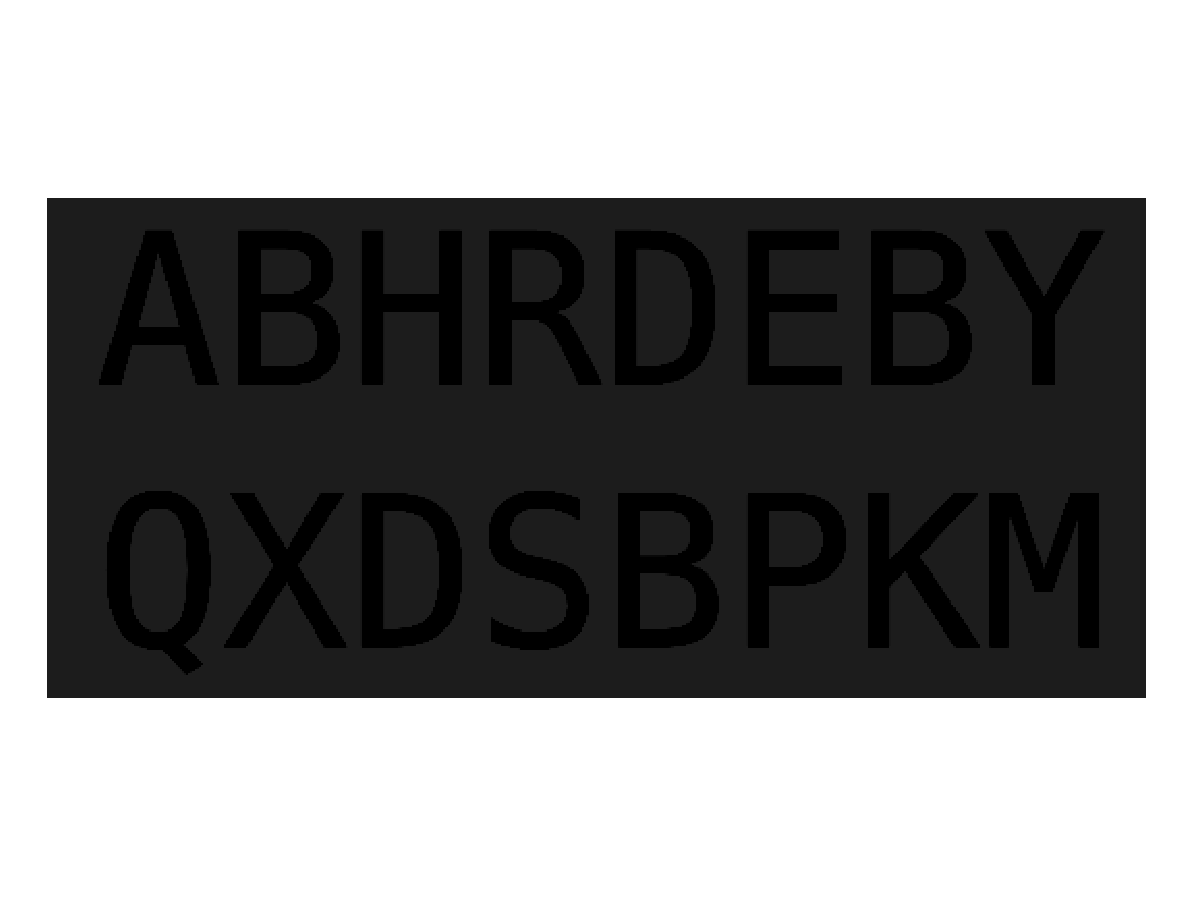
\includegraphics[scale=0.18]{illus/motm0.png}\\
			Motif en niveaux de gris avec valeur moyenne nulle  & Image en niveaux de gris avec valeur moyenne nulle\\
	\end{tabular}
	\subsection{La recherche}
	Maintenant que nos images sont prêtes on peut commencer à chercher le motif dans l'image. Pour cela nous allons utiliser l'intercorrélation. En calculant les coefficients de corrélation entre les deux images, on va pouvoir localiser où le motif original a été translaté horizontalement ou verticalement.
	Sur \octave nous utilisons la fonction \texttt{normxcorr2} afin d'obtenir les coefficients de corrélation normalisés. Cette fonction renvoie une matrice, d'une taille supérieure à l'image, contenant les coefficients, plus le coefficient est proche de 1, plus le motif est semblable à la partie de l'image analysée.
	Nous pouvons représenter cette matrice sur un graphe et ainsi repérer les points de similitude.\\
	\begin{tabular}{|c|c|}
			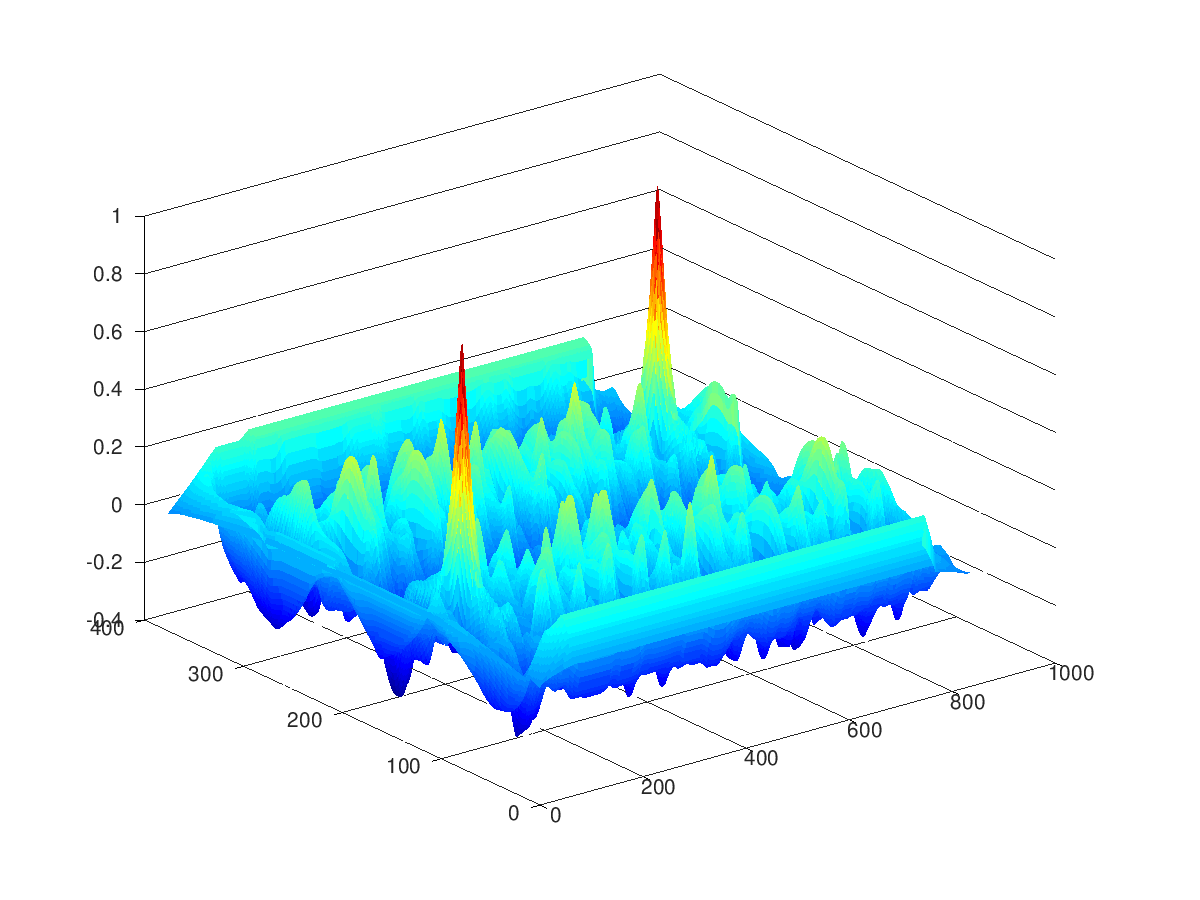
\includegraphics[scale=0.18]{illus/cor.png} & 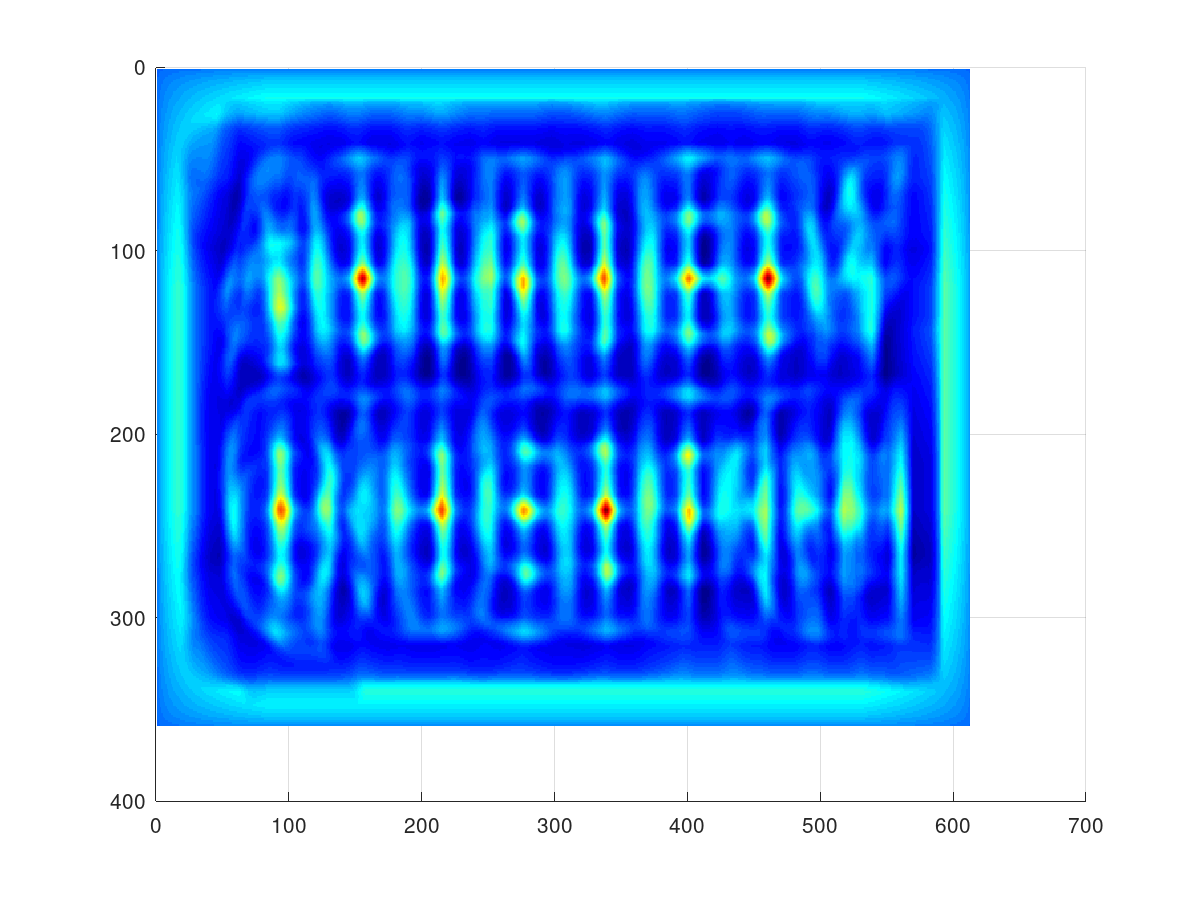
\includegraphics[scale=0.18]{illus/cor1.png}\\
			Représentation des coefficients en 3D  & Représentation des coefficients vue de dessous\\
	\end{tabular}
	Avec ces représentations, nous pouvons repérer les occurrences du motif dans l'image. Il faut maintenant récupérer les coordonnées des pics les plus hauts pour localiser le motif.
	\subsection{L'affichage}
	\section{Fonctionnement}	
	
	\section{Problèmes restants}
	Taille caractère
	postition des cercles de localisation
	\section*{Conclusion}
\end{document}